\documentclass[handout]{beamer}

\usetheme[progressbar=frametitle]{metropolis}
\metroset{block=fill}

\subtitle{NTIN071 Automata and Grammars}
\author{Jakub Bulín (KTIML MFF UK)}

\date{Spring 2025\\ 
    \vspace{1in} 
    \begin{flushleft}
        \it \footnotesize * Adapted from the Czech-lecture slides by Marta Vomlelová with gratitude. The translation, some modifications, and all errors are mine.
    \end{flushleft}
}

%% packages

\usepackage{amsmath}
\usepackage{amssymb}
\usepackage{amsthm}
\usepackage{cancel}
\usepackage{color}
\usepackage{colortbl}
\usepackage{forest}
\usepackage[utf8x]{inputenc}
\usepackage{multicol}
\usepackage{multirow}

%% colors
\definecolor{Gray}{gray}{0.9}

%% TikZ
\usepackage{tikz}
    \usetikzlibrary{
        automata,
        arrows,
        backgrounds,
        decorations.pathmorphing,
        fit,
        positioning,
        shapes,
        shapes.geometric,
        tikzmark
    } 
    \tikzset{>=stealth',shorten >=1pt,auto,node distance=2cm}
    \tikzset{initial text={}}
    \tikzset{elliptic state/.style={draw,ellipse}}

%% amsthm
\theoremstyle{plain}
    \newtheorem*{algorithm}{Algorithm}    
    \newtheorem*{observation}{Observation}
    \newtheorem*{proposition}{Proposition}

\theoremstyle{remark}
    \newtheorem*{exercise}{Exercise}
    \newtheorem*{remark}{Remark}

%% macros
\DeclareMathOperator{\RegE}{RegE}
\DeclareMathOperator{\RL}{RL}

% Just for Lecture 2
\newcommand{\x}{$\times$}
\newcommand{\nx}{\ }



\title{Lecture 7 -- Pushdown automata}


\begin{document}


\frame{\titlepage}


\begin{frame}{Recap of Lecture 6}
	
    \begin{itemize}
		\item Reducing a grammar: removing $\epsilon$-productions, unit productions, useless symbols
		\item Chomsky Normal Form of a context-free grammar
		\item Pumping lemma for context-free languages, application: proving non-context-freeness
		\item Testing membership in a context-free language: the CYK algorithm
	\end{itemize}
	
\end{frame}


\section{2.9 Pushdown automata}


\begin{frame}{Pushdown automaton (PDA)}

    \vspace{-6pt}
    \begin{center}
        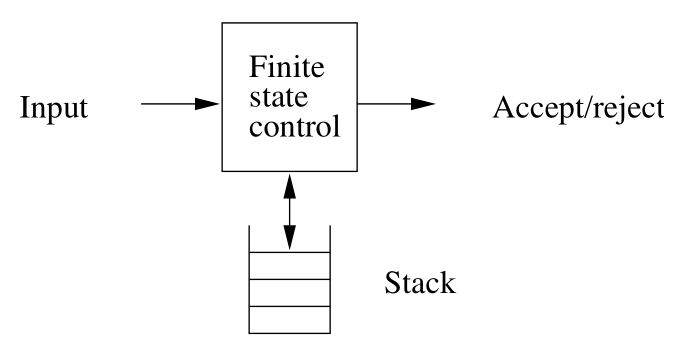
\includegraphics[width=0.6\textwidth]{files/pushDown.PNG}
    \end{center}
    \vspace{-12pt}

    \begin{itemize}
        \item an extension of $\epsilon$--NFA, additional feature: a \alert{stack} memory %(push, pop -- only at the top)
        \item the stack has its own \alert{stack alphabet} $\Gamma$ (can contain $\Sigma$ or not)
        \item at each step we pop the top stack symbol $X$, make a decision based on $(q,a,X)$, push some word $\gamma\in\gamma^*$
        \item the stack can rememeber an infinite amount of information
        \item PDA define context-free languages, nondeterminism is important: \alert{deterministic} PDA only recognize a proper subset of context-free languages (unlike DFA vs. NFA)
    \end{itemize}
    
\end{frame}


\begin{frame}{The definition}

    \alert{A pushdown automaton} (\alert{PDA}): $P=(Q,\Sigma,\Gamma,\delta,q_0,Z_0,F)$, where
        
    \begin{itemize}
        \item $Q$ is finite, nonempty set of states
        \item $\Sigma$ is a finite, nonempty \alert{input alphabet}
        \item $\Gamma$ is a finite, nonempty \alert{stack alphabet}
        \item $\delta$ is the \alert{transition function}, 
        $$
        \delta\colon Q\times (\Sigma\cup \{\epsilon\})\times \Gamma \to \mathcal P_{FIN}(Q \times \Gamma^*)
        $$ 
        $\delta(q,a,X)\ni(p,\gamma)$ where $p$ is the new state and $\gamma$ a finite string of stack symbols that \alert{replace} $X$ on top of the stack
        \item $q_0\in Q$ is the \alert{initial state}
        \item $Z_0\in\Gamma$ is the \alert{initial stack symbol} (\alert{bottom of the stack}); the only symbol on the stack at the beginning
        \item $F$ is a set of \alert{accepting} (\alert{final}) states; may be undefined if our PDA \alert{accepts by empty stack}
    \end{itemize}

\end{frame}


\begin{frame}{One transition of a PDA}   

    \begin{itemize}
        \item read one input letter ($a\in\Sigma$) or do an $\epsilon$-transition ($a=\epsilon$)
        \item pop $X$ from the top of the stack
        \item based on $a$, $X$, and the current state $q$ nondeterministically choose one of finitely many options $(p,\gamma)\in\delta(q,a,X)$
        \item switch to the new state $p$
        \item push the finite string $\gamma$ to the stack (the first symbol of $\Gamma$ is now on top)
        \item \alert{pop}: $\gamma=\epsilon$, \alert{read} only: $\gamma=X$, \alert{push}: $\gamma=\gamma'X$
\end{itemize}

\end{frame}


\begin{frame}{An example: $L=\{ww^R\mid w \in \{0,1\}^*\}$}

    \begin{center}

        \scalebox{0.95}{
        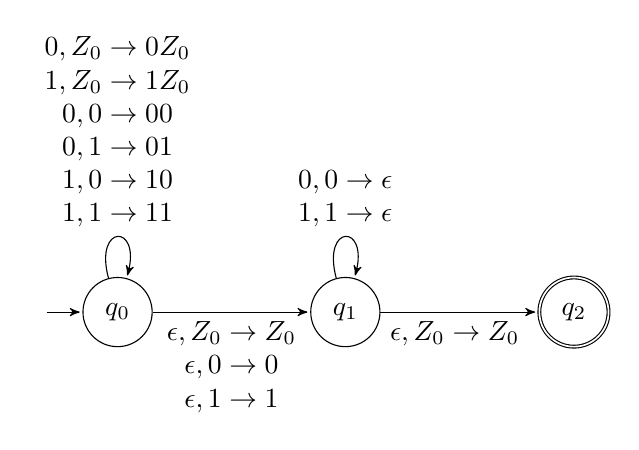
\begin{tikzpicture}[]
            \node[initial,state] (q0)      {$q_0$};
            \node[state] (q1)  [right=2cm of q0]     {$q_1$};
            \node[state, accepting] (q2)  [right=2cm of q1]    {$q_2$};
            \path[->]
                (q0)  edge[loop above]  node[align=center] {
                                        $0,Z_0 \rightarrow 0Z_0$	\\
                                        $1,Z_0 \rightarrow 1Z_0$	\\			
                                        $0,0 \rightarrow 00$	\\			
                                        $0,1 \rightarrow 01$	\\			
                                        $1,0 \rightarrow 10$	\\			
                                        $1,1 \rightarrow 11$			
                                        } (q0)
                (q0)  edge[swap]  node[align=center] {
                                        $\epsilon,Z_0 \rightarrow Z_0$	\\			
                                        $\epsilon,0 \rightarrow 0$	\\			
                                        $\epsilon,1 \rightarrow 1$			
                                        }  (q1)
                (q1)  edge[loop above]  node[align=center] {
                                        $0,0 \rightarrow \epsilon$	\\			
                                        $1,1 \rightarrow \epsilon$			
                                        } (q1)
                (q1)  edge[swap]  node[align=center] {
                                        $\epsilon,Z_0 \rightarrow Z_0$	
                                        } (q2)
                ;
        \end{tikzpicture}
        }
    \end{center}

    \vspace{-12pt}   
    
    \alert{$q_0$} read input letters pushing them onto the stack; guess the middle (nondeterministically), jump to $q_1$\\
    \alert{$q_1$} compare input with stack, consuming both; if empty stack (we see the bottom), accept by jumping to $q_2$; no input can remain

\end{frame}


\begin{frame}{Example cont'd: full description of the PDA}

    \begin{center}
        $P=(\{q_0,q_1,q_2\},\{0,1\},\{0,1,Z_0\},\delta,q_0,Z_0,\{q_2\})$
    \end{center}

    \begin{tabular}{l l}\hline
        $\delta(q_0,0,Z_0)=\{(q_0,0Z_0)\}$ &  
            \multirow{2}{*}{push input onto stack, leave the bottom} \\
        $\delta(q_0,1,Z_0)=\{(q_0,1Z_0)\}$ &  \\\hline
        $\delta(q_0,0,0)=\{(q_0,00)\}$ &  
            \multirow{4}{*}{stay in $q_0$, push input onto stack}\\ 
        $\delta(q_0,0,1)=\{(q_0,01)\}$ \\
        $\delta(q_0,1,0)=\{(q_0,10)\}$ \\
        $\delta(q_0,1,1)=\{(q_0,11)\}$ \\ \hline
        $\delta(q_0,\epsilon,Z_0)=\{(q_1,Z_0)\}$ &
            \multirow{3}{*}{jump to $q_1$ without changing stack}\\ 
        $\delta(q_0,\epsilon,0)=\{(q_1,0)\}$ \\
        $\delta(q_0,\epsilon,1)=\{(q_1,1)\}$ \\ \hline
        $\delta(q_1,0,0)=\{(q_1,\epsilon)\}$ &
            \multirow{2}{*}{pop stack and match with input}\\ 
        $\delta(q_1,1,1)=\{(q_1,\epsilon)\}$ \\ \hline
        $\delta(q_1,\epsilon,Z_0)=\{(q_2,Z_0)\}$ & we have $ww^R$, go to accepting state
        \\\hline
        \end{tabular}

\end{frame}


\end{document}


\begin{frame}{Notation}

    \begin{definition}[Transition diagram for PDA]
        A transition diagram for PDA contains:
        \begin{itemize}
            \item The nodes correspond to the states of the PDA.
            \item The first arrow indicates the start state, and doubly circled states are accepting.
            \item The arc correspond to transitions of the PDA. An arc labeled $a,X\rightarrow \alpha $ from state $q$ to $p$ means that $\delta(q,a,X)\ni (p,\alpha)$.
            \item Conventionally, the start stack symbol is $Z_0$.
        \end{itemize}
        \end{definition}



{
    Labels:\\
     input\_symbol, stack\_symbol $\rightarrow$ string\_to\_push \\[0.5cm]
    }
    
    \vspace{1.5cm}
    
    \begin{center}
    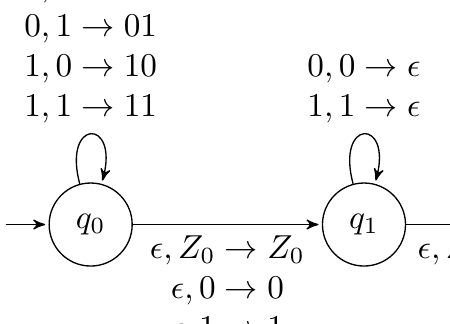
\begin{tikzpicture}[]
    \useasboundingbox (-0.8,-0.9) rectangle (4.2,2.5);
        \scope[transform canvas={scale=1.2}]
                \node[initial,state] (q0)      {$q_0$};
                \node[state] (q1)  [right=2cm of q0]     {$q_1$};
                \node[state, accepting] (q2)  [right=2cm of q1]    {$q_2$};
            \path[->]
                    (q0)  edge[loop above]  node[align=center] {
                                    $0,Z_0 \rightarrow 0Z_0$	\\
                                    $1,Z_0 \rightarrow 1Z_0$	\\			
                                    $0,0 \rightarrow 00$	\\			
                                    $0,1 \rightarrow 01$	\\			
                                    $1,0 \rightarrow 10$	\\			
                                    $1,1 \rightarrow 11$			
                                    } (q0)
                    (q0)  edge[swap]  node[align=center] {
                                    $\epsilon,Z_0 \rightarrow Z_0$	\\			
                                    $\epsilon,0 \rightarrow 0$	\\			
                                    $\epsilon,1 \rightarrow 1$			
                                    }  (q1)
                    (q1)  edge[loop above]  node[align=center] {
                                    $0,0 \rightarrow \epsilon$	\\			
                                    $1,1 \rightarrow \epsilon$			
                                    } (q1)
                    (q1)  edge[swap]  node[align=center] {
                                    $\epsilon,Z_0 \rightarrow Z_0$	
                                    } (q2)
                    ;
        \endscope
    \end{tikzpicture}
    \end{center}

\end{frame}


\end{document}


\subsection*{Graphical notation for PDA's}

\begin{definition}[Transition diagram for PDA]
A transition diagram for PDA contains:
\begin{itemize}
	\item The nodes correspond to the states of the PDA.
	\item The first arrow indicates the start state, and doubly circled states are accepting.
	\item The arc correspond to transitions of the PDA. An arc labeled $a,X\rightarrow \alpha $ from state $q$ to $p$ means that $\delta(q,a,X)\ni (p,\alpha)$.
	\item Conventionally, the start stack symbol is $Z_0$.
\end{itemize}
\end{definition}



{
Labels:\\
 input\_symbol, stack\_symbol $\rightarrow$ string\_to\_push \\[0.5cm]
}

\vspace{1.5cm}

\begin{center}
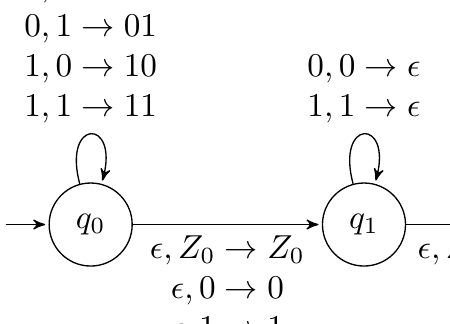
\begin{tikzpicture}[]
\useasboundingbox (-0.8,-0.9) rectangle (4.2,2.5);
    \scope[transform canvas={scale=1.2}]
			\node[initial,state] (q0)      {$q_0$};
			\node[state] (q1)  [right=2cm of q0]     {$q_1$};
			\node[state, accepting] (q2)  [right=2cm of q1]    {$q_2$};
		\path[->]
				(q0)  edge[loop above]  node[align=center] {
								$0,Z_0 \rightarrow 0Z_0$	\\
								$1,Z_0 \rightarrow 1Z_0$	\\			
								$0,0 \rightarrow 00$	\\			
								$0,1 \rightarrow 01$	\\			
								$1,0 \rightarrow 10$	\\			
								$1,1 \rightarrow 11$			
								} (q0)
				(q0)  edge[swap]  node[align=center] {
								$\epsilon,Z_0 \rightarrow Z_0$	\\			
								$\epsilon,0 \rightarrow 0$	\\			
								$\epsilon,1 \rightarrow 1$			
								}  (q1)
				(q1)  edge[loop above]  node[align=center] {
								$0,0 \rightarrow \epsilon$	\\			
								$1,1 \rightarrow \epsilon$			
								} (q1)
				(q1)  edge[swap]  node[align=center] {
								$\epsilon,Z_0 \rightarrow Z_0$	
								} (q2)
				;
    \endscope
\end{tikzpicture}
\end{center}


\subsection*{Notation Convention for PDA's}
\begin{center}
	\begin{tabular}{l l}
$a,b,c$ & symbols of the input alphabet\\
$q,p, r_\ell$ & states\\
$u,w,x,y,z$ & strings of input symbols\\
$X,Y,E,Z_0$ & stack symbols\\
$\alpha,\beta,\gamma$ & strings of stack symbols.		
	\end{tabular}
\end{center}

\bigskip


\section*{The Languages of a PDA}


\subsection*{Describing computation}

\begin{definition}[PDA situation, ID]
We represent the situation of a PDA by a triple $(q,w,\gamma)$, where
\begin{description}
	\item[$q$] is the state 
	\item[$w$] is the remaining input and
	\item[$\gamma$] is the stack contents (top on the left). 
\end{description}
Such a tripple is called an \alert{instantaneous description (ID), situation} of the pushdown automaton.
\end{definition}
\begin{definition}[$\vdash,\vdash^*$ PDA Computation, Sequences of situations]
Let $P=(Q,\Sigma,\Gamma,\delta,q_0,Z_0,F)$ be a PDA. Define $\vdash_P$ or just $\vdash$ as follows. Suppose $\delta(q,a,X)\ni(p,\alpha)$. Then for all strings $w\in \Sigma^*$ and $\beta\in \Gamma^*$:
$$(q,aw,X\beta)\vdash (p,w,\alpha\beta)\hbox{.}
$$
We also use the symbol $\vdash^*_P$ or $\vdash^*$ to represent zero or more moves of the PDA, i.e.
\begin{itemize}
	\item $I\vdash^*I$ for any ID $I$
	\item $I\vdash^*J$ if there exists some ID $K$ such that $I\vdash K$ and $K\vdash^*J$.
\end{itemize}
\end{definition}

\newcommand{\carka}{,}
\begin{example}[ID's of the PDA on input $1111$]

\bigskip

\hspace{-5cm}
\begin{forest}
for tree={edge=->}
[$(q_0\carka 1111\carka Z_0)$
	[$(q_0\carka 111\carka 1Z_0)$
	[$(q_0\carka 11\carka 11Z_0)$
	[$(q_0\carka 1\carka 111Z_0)$
	[$(q_0\carka \epsilon\carka 1111Z_0)$[$(q_1\carka \epsilon\carka 1111Z_0)$]]
	[$(q_1\carka 1\carka 111Z_0)$[$(q_1\carka \epsilon\carka 11Z_0)$]]]
	[$(q_1\carka 11\carka 11Z_0)$[$(q_1\carka 1\carka 1Z_0)$[$(q_1\carka \epsilon\carka Z_0)$[$(q_2\carka \epsilon\carka Z_0)$,tikz={\node [draw,green,fit=()] {};}]]]]
	]
[$(q_1\carka 111\carka 1Z_0)$[$(q_1\carka 11\carka Z_0)$[$(q_2\carka 11\carka Z_0)$]]]
]
[$(q_1\carka 1111\carka Z_0)$[$(q_2\carka 1111\carka Z_0)$]]
]
%[$(q_0\carka 1111)$]
\end{forest}
\end{example}

\bigskip

\subsection*{Acceptance by Final State}

\begin{definition}[PDA language accepted by final state]
Let $P=(Q,\Sigma,\Gamma,\delta,q_0,Z_0,F)$ be a PDA. Then $L(P)$,
the \alert{language accepted by $F$ by a final state}, is
 $$L(P)=\{w |(q_0,w,Z_0)\vdash^*_P (q,\epsilon,\alpha) \hbox{ for some } q\in F \hbox{ and any stack string }\alpha \}\hbox{.}$$
\end{definition}
\begin{example}
The PDA example for $L_{wwr}$ accepts the language.
\end{example}
\begin{itemize}
	\item (IF) For any $x=ww^R$, we have a accepting computation
	$$(q_0,ww^R,Z_0)\vdash^*(q_0,w^R,w^RZ_0)\vdash (q_1,w^R,w^RZ_0)\vdash^*(q_1,\epsilon,Z_0)\vdash(q_2,\epsilon,Z_0)\hbox{.} $$
	\item (Only If) 
\begin{itemize}
	\item 	The only way to enter $q_2$ is from $q_1$ and $Z_0$ at the top of the stack.
	\item Any accepting computation starts in $q_0$, changes to $q_1$ and never returns to $q_0$.
	\item We can prove by induction on $|x|$ that $(q_0,x,Z_0)\vdash^*(q_1,\epsilon,Z_0)$ exactly for the strings of the form $x=ww^R$. 
\end{itemize}
\end{itemize}



\bigskip
\subsection*{Acceptance by Empty Stack}
\begin{definition}[PDA language accepted by empty stack]
For each PDA $P=(Q,\Sigma,\Gamma,\delta,q_0,Z_0{\color{orange},F})$ we define 
 $N(P)$,the \alert{language accepted by $P$ by empty stack}
 $$N(P)=\{w |(q_0,w,Z_0)\vdash^*_P (q,\epsilon,\epsilon) \hbox{ for some }q\in Q\}\hbox{.}$$

The set of accepting states is in this case irrelevant, we shall sometimes leave it off and state $P$ as a six-tuple $P=(Q,\Sigma,\Gamma,\delta,q_0,Z_0)$.
\end{definition}
\begin{example}
In the previous example, we change the transition $\delta(q_1,\epsilon,Z_0)=\{(q_2,Z_0)\}$ to pop the last symbol: $\delta(q_1,\epsilon,Z_0)=\{(q_2,\epsilon)\}$. Now, $L(P')=N(P')=L_{wwr}$.
\end{example}

